\chapter{Introduction}
Traditionally, radar systems consisted of discrete components with high system
cost and power consumption, but recent development of integrated single-chip
Frequency Modulated Continuous Wave (FMCW) radars significantly reduce the cost,
size, and power consumption of these systems. These
integrated CMOS FMCW radar systems operate at 76-81 GHz, with radial range resolutions
as high as 3.75 cm due to sweep bandwidths up to 4 GHz and velocity resolutions
as high as 0.05 m/s. Due to regulations and available bandwidths,
previous radar systems operating at lower frequencies ($<24$ GHz) have smaller
sweep bandwidths, leading to reduced range resolutions and reduced velocity
resolutions, due to the larger carrier wavelengths. Given these recent developments in
high-frequency, wide-band radar, we predict that these radar devices will
revolutionize wireless sensing and imaging capabilities. 

Modern vehicles are equipped with a wide variety of available data, including
vehicle odometry, and in recent years cars have been equipped with cameras and
radar for features like collision detection and Traffic Aware Cruise Control.

\begin{figure}[h]
	\centering
	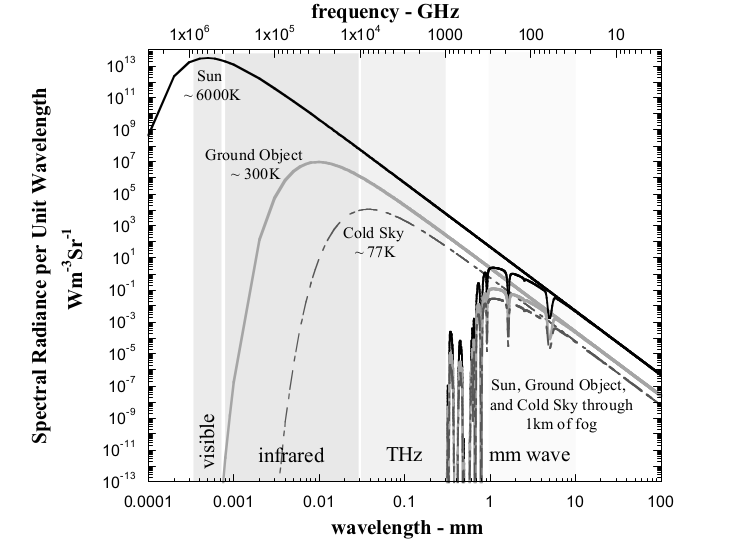
\includegraphics[width=0.8\textwidth]{imgs/attenuation}
	\caption{Loss bands within millimeter wave region allow for sensing in
	adverse weather conditions \cite{patel2016computational}.}
	\label{fig:attentuation}
\end{figure}

In recent years, the computer vision community has made dramatic progress on classification,
detection, tracking, and other problems with the development of deep neural
networks, using large labeled training datasets. However, vision alone cannot
solve certain problems such as position and velocity measurements with
satisfactory results, but radar systems excel at these. Additionally, the
presence of environmental conditions, such as rain, fog, smoke, and dust
significantly hinder visible system performances, but radar performance is
relatively unaffected in these situations \cite{patel2016computational}. Figure \ref{fig:attentuation} shows the atmospheric
attenuation of naturally emitted black-body radiation through 1 km of fog. 

In this thesis, we will cover the mathematics for determing range, velocity, and
estimating angle of arrival for targets in front of a FMCW radar. 
